
\documentclass{beamer}

\usepackage{xargs}
\usepackage{tikz}

\colorlet{darkred}{red!80!black}

\tikzset{->-/.style={decoration={
  markings,
  mark=at position 1 with {\arrow{>}}},postaction={decorate}}}
\tikzset{-<-/.style={decoration={
  markings,
  mark=at position 0.2 with {\arrow{<}}},postaction={decorate}}}

\definecolor{thegrey1}{rgb}{.72,.72,.72}
\definecolor{thegrey2}{rgb}{.50,.50,.50}
\definecolor{theblue}{rgb}{0,.24,.98}

\tikzstyle{nclnode}=[draw=thegrey2,fill=thegrey1,circle,inner sep=0pt, minimum size=4pt]
\tikzstyle{ncl1}=[line cap=round,line width=1.5pt,darkred]
\tikzstyle{ncl2}=[line cap=round,line width=3pt,theblue]

\begin{document}



%--------------------------------
\begin{frame}

\[
\scalebox{1.6}{
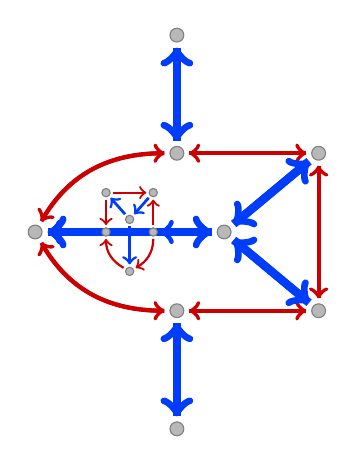
\begin{tikzpicture}[x=6mm,y=10mm]
	\foreach \a/\p in 
		{a/{(0,2)},b/{(3,3)},c/{(3,1)},d/{(6,3)},e/{(6,1)},f/{(4,2)},1/{(3,4.5)},0/{(3,-.5)}}
		{\node[nclnode,minimum size=5pt,outer sep=2pt] (\a) at \p {};}
	%
	\begin{scope}[ncl1,->,cap = butt]
	  \draw<1-2> (a) to[out=60,in=180] (b);  \draw<3-> (b) to[out=180,in=60] (a);
	  \draw<1-8> (c) to[in=300,out=180] (a); \draw<9-> (a) to[out=300,in=180] (c);
	  \draw<1-2> (d) -- (b); \draw<3-> (b) -- (d);
	  \draw<1-8> (c) -- (e); \draw<9-> (e) -- (c);
	  \draw<1-5> (d) -- (e); \draw<6-> (e) -- (d);
	\end{scope}
	%
	\begin{scope}[ncl2,->,cap = butt]
	  \draw<1-3,8-10> (f) -- (a); \draw<4-7> (a)--(f);
	  \draw<1>   (b) -- (1); \draw<2-> (1)--(b);
	  \draw<1-9> (0) -- (c); \draw<10->(c)--(0);
	  \draw<1-6> (f) -- (d); \draw<7-> (d)--(f);
	  \draw<1-4> (e) -- (f); \draw<5-> (f)--(e);
	\end{scope}
	%
	\foreach \a/\p in 
		{a1/{(2,1.5)},b1/{(1.5,2)},c1/{(2.5,2)},d1/{(1.5,2.5)},e1/{(2.5,2.5)},f1/{(2,2.16)}}
		{\node<11>[nclnode,minimum size=3pt,outer sep=1pt] (\a) at \p {};}
	%
	\begin{scope}[ncl1,line width=.8pt,->,cap = butt]
	  \draw<11> (a1) to[out=150,in=270] (b1); 
	  \draw<11> (c1) to[in=30,out=270] (a1);
	  \draw<11> (d1) -- (b1);
	  \draw<11> (c1) -- (e1);
	  \draw<11> (d1) -- (e1);
	\end{scope}
	%
	\begin{scope}[ncl2,line width=1pt,->,cap = butt]
	  \draw<11> (f1) -- (a1);
	  \draw<11> (f1) -- (d1);
	  \draw<11> (e1) -- (f1);
	\end{scope}
	\draw<11>[ncl2,->,line width=2pt,cap = butt] (b1) -- (a);
	\draw<11>[ncl2,->,line width=2pt,cap = butt] (f) -- (c1);
	%
\end{tikzpicture}
}
\]

\end{frame}

\end{document}




